%----------------------------------------------------------%
% Beamer template for presentations within PPGCC PUCRS     %
% by Anderson Domingues (anderson.domingues@acad.pucrs.br) %
%                                                          %
% made over "Template Beamer para Apresentações da UFRN"   %
% by alcemygvseverino@gmail.com (ver. 1.1, 14/05/2016)     %
%----------------------------------------------------------%

\documentclass[aspectratio=169,handout,t,table]{beamer}

%\usepackage[table]{xcolor}
\usepackage[english]{babel}              % document language
\usepackage[utf8]{inputenc}              % utf-8 support
% \usepackage{multicol}

%\usepackage[alf]{abntex2cite}            % ABNT citation style

\usepackage[square, sort, comma, numbers]{natbib}
\usepackage{graphicx}
\usepackage{float}
\usepackage{geometry}
\usepackage{tikz}
\usepackage{amsmath}
\usepackage{amssymb}

\usepackage{multirow}

% \usepackage{url}
\usepackage{pgfpages}                   % allows including pdf

\usepackage{enumerate}
\usepackage{color}
\usepackage{ifthen}
\usepackage{capt-of}                    % support for caption 

\usepackage{soul}
\usepackage{booktabs}

\usepackage{pgfplots}
\usepackage{pgfplotstable}
\usepackage{svg}


% Background
% \setbeamertemplate{background}{
%     \includegraphics[width=\paperwidth,keepaspectratio]{template/sbcci24bg.png}
% }

% TikZ solution
\newcommand*\circnum[1]{\tikz[baseline=(char.base)]{
            \node[shape=circle,draw,inner sep=1.2pt] (char) {#1};}} 

\usetikzlibrary{arrows,shapes,fit,positioning,shadows,trees,calc,pgfplots.groupplots}
\tikzset{every picture/.style={/utils/exec={\sffamily}}}
\definecolor{omni-spring-pastels-1}{HTML}{fd7f6f}
\definecolor{omni-spring-pastels-2}{HTML}{7eb0d5}
\definecolor{omni-spring-pastels-3}{HTML}{b2e061}
\definecolor{omni-spring-pastels-4}{HTML}{bd7ebe}
\definecolor{omni-spring-pastels-5}{HTML}{ffb55a}
\definecolor{omni-spring-pastels-6}{HTML}{ffee65}
\definecolor{omni-spring-pastels-7}{HTML}{beb9db}
\definecolor{omni-spring-pastels-8}{HTML}{fdcce5}
\definecolor{omni-spring-pastels-9}{HTML}{8bd3c7}


\usetheme{Berlin}                       % theme (layout)
\usecolortheme{pucrs}                    % colors

\setbeamertemplate{caption}[numbered]   % add enumeration to figures

\title[Joint Computation and Communication Analysis of Hard Real-Time applications in Manycores]{% TITLE
Joint Computation and Communication Analysis of Hard Real-Time applications in Manycores}

\author[Angelo Elias Dal Zotto]{Anderson R. P. Domingues, Lucas Damo, Sergio J. Filho, and Fernando G. Moraes \newline
\footnotesize{\{anderson.domingues, lucas.damo\}@edu.pucrs.br; \{sergio.filho, fernando.moraes\}@pucrs.br}}

\institute[PUCRS]{
PUCRS – School of Technology, Porto Alegre, Brazil\\\vspace{1em}
Presenter: \textbf{Angelo Dal Zotto}}

\titlegraphic{
    \vspace{1cm}
    \includegraphics[height=1cm]{template/gaph.png}
    \hspace*{\fill}
    \includegraphics[height=1cm]{template/sbcci24.png}
    \hspace*{\fill}
    \includegraphics[height=1.2cm]{template/pucrs.png}
}

\logo{
    \includegraphics[height=1cm, decodearray={0.85 1 0.85 1 0.85 1}]{template/sbcci24bw.png}
}

\begin{document}

\AtBeginSection[]
{
    \begin{frame}
        \frametitle{Overview}
        % \begin{multicols}{2}
            % \tableofcontents[currentsection, hideothersubsections]
        % \end{multicols}
        \tableofcontents[hideallsubsections]
    \end{frame}
}

\frame[plain]{\titlepage}

% your content goes below
\section{Introduction}

\begin{frame}{Introduction}
    \begin{itemize}
        \item Manycore systems are intrinsic to modern interconnected environments, particularly in IoT networks. 
        
        \item However, this interconnectivity renders them \textbf{susceptible to various forms of cyberattacks}.
        
        \item The use of third-party intellectual property cores as a solution to cope with design complexity and time-to-market pressures further worsens these vulnerabilities.
        
        \item Security is a critical concern in developing and deploying manycore systems.

        \item The existing literature offers various strategies for threat \ul{\textit{detection}} \cite{Charles:2021:Survey}, \ul{\textit{localization}} of these threats \cite{Subodha:2020:Localization}, and the corresponding \ul{\textit{countermeasures}} \cite{Faccenda:2021:Countermeasures} in NoC-based manycores. This work focuses on \textbf{threat detection}.  
    \end{itemize}
\end{frame}

\begin{frame}{Related Work}
    
    \begin{itemize}
    
    \item Early research: ad-hoc algorithms based on exclusive latency monitoring, such as RLAN \cite{Rajesh2015}, that cannot account for variations such as in application mapping.
    
    \item Kulkarni et al. \cite{Kulkarni:2016:SVM} presents one of the first ML proposals for anomaly detection in manycore systems. The Authors assess diverse ML algorithms and choose SVM as their implementation in FPGA. This implementation employs synthetic traffic generated by an external data injector, which does not accurately represent real-world workloads. 
                    
    \end{itemize}
\end{frame}

\begin{frame}{Related Work}
    
    \begin{itemize}
                    
    \item Sudusinghe et al. propose methods for detecting flooding DoS \cite{Sudusinghe:2021:DoS} and eavesdropping attacks \cite{Sudusinghe:2022:Eevesdropping} using ensemble learners. Routers in their systems have probes that send relevant features to centralized detectors. The Authors evaluate their work with Gem5.

    \item TSA-NoC \cite{Wang:2020:TSA-NoC} and AGAPE \cite{Wang:2022:AGAPE} detect HTs using Neural Networks (NN). These approaches have as a drawback the NN area overhead, which every NoC router incorporates.
    
    \end{itemize}
\end{frame}


\begin{frame}{Problem}
    \begin{itemize}

    \item Limitations found in early work on threat localization and in works using ML.

    \begin{itemize}
        \item \ul{\textit{applicability}}, is due to costly techniques, usually based on NN, replicated at every router in the NoC \cite{Rajesh2015, Wang:2020:TSA-NoC, Wang:2022:AGAPE, Sinha:2021:Sniffer}. 

        \ul{\textit{confidence}}, is due to the adoption of synthetic NoC traffic that does not represent real application scenarios \cite{Kulkarni:2016:SVM, Madden:2018:NN, Vashist:2019:WiNoC, Yao:2020:Localization, Hu:2023:Cascaded} and the use of high-level simulators \cite{Sudusinghe:2021:DoS, Sudusinghe:2022:Eevesdropping, Wang:2020:TSA-NoC, Wang:2022:AGAPE, Sinha:2021:Sniffer, Madden:2018:NN, Yao:2020:Localization, Hu:2023:Cascaded}, such as Gem5, which do not reflect the actual accuracy of the systems.
    \end{itemize}
        
    \end{itemize}
\end{frame}

\begin{frame}{Proposed solution}
    \begin{itemize}    
    
    \item Goals: \begin{itemize}
        \item detect anomalies in the NoC traffic caused by malicious sources, characterizing a security threat
        \item using an ML flow that profiles real applications in an actual manycore, modeled at the RTL level with clock cycle accuracy.
    \end{itemize}

    \item Original contributions \begin{itemize}
        \item create and use application profiles instead of synthetic NoC traffic

        \item detect subtle, uncorrelated traffic collisions that occur due to disturbing malicious traffic in applications.
    \end{itemize}
    
    \end{itemize}
\end{frame}

\section{Baseline Platform}

\begin{frame}{Application profile}
    \centering Example with MPEG application (pipeline)
    \begin{figure}[!ht]
        \centering
        \resizebox{.5\linewidth}{!}{
            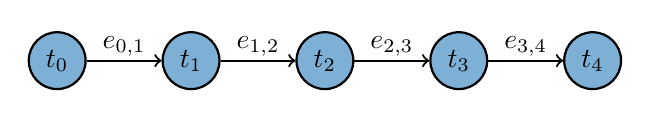
\begin{tikzpicture}[thick, node distance={17mm}, main/.style={circle,draw,fill=omni-spring-pastels-2}]
    
    \node[main] (4) {$t_0$};
    \node[main] (2) [right of=4] {$t_1$};
    \node[main] (1) [right of=2] {$t_2$};
    \node[main] (0) [right of=1] {$t_3$};
    \node[main] (3) [right of=0] {$t_4$};
    
    \draw[->] (4) -- (2) node[midway, yshift=5] {$e_{0,1}$};
    \draw[->] (2) -- (1) node[midway, yshift=5] {$e_{1,2}$};
    \draw[->] (1) -- (0) node[midway, yshift=5] {$e_{2,3}$};
    \draw[->] (0) -- (3) node[midway, yshift=5] {$e_{3,4}$};
    
\end{tikzpicture}

        }
    \end{figure}
    
    \vspace{10pt}
    \begin{columns}
        \column{.45\linewidth}
        \centering Contiguous mapping
        \begin{figure}
            \centering
            \resizebox{.4\linewidth}{!}{
                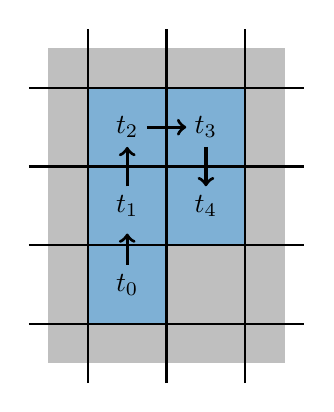
\begin{tikzpicture}[thick]
    \fill[gray!50](0.5,0.5) rectangle (3.5, 4.5); ;
    \draw[step=1 cm, color=black] (0.25, 0.25) grid (3.75, 4.75);
    
    \node[fill=omni-spring-pastels-2, minimum size=1 cm, draw=black] (1) at (1.5, 1.5) {\textbf{$t_0$}};
    \node[fill=omni-spring-pastels-2, minimum size=1 cm, draw=black] (3) at (1.5, 2.5) {\textbf{$t_1$}};
    \node[fill=omni-spring-pastels-2, minimum size=1 cm, draw=black] (2) at (1.5, 3.5) {\textbf{$t_2$}};
    \node[fill=omni-spring-pastels-2, minimum size=1 cm, draw=black] (4) at (2.5, 3.5) {\textbf{$t_3$}};
    \node[fill=omni-spring-pastels-2, minimum size=1 cm, draw=black] (5) at (2.5, 2.5) {\textbf{$t_4$}};
    

    \coordinate (2t1) at (1.5, 2.75) ;
    \coordinate (1f2) at (1.5, 3.25) ;
    \draw[->, very thick] (2t1) -- (1f2);
    
    \coordinate (4t2) at (1.5, 1.75) ;
    \coordinate (2f4) at (1.5, 2.15) ;
    \draw[->, very thick] (4t2) -- (2f4);

    \coordinate (1t0) at (1.75, 3.5) ;
    \coordinate (0f1) at (2.25, 3.5) ;
    \draw[->, very thick] (1t0) -- (0f1);
    
    
    \coordinate (0t3) at (2.5, 3.25) ;
    \coordinate (3f0) at (2.5, 2.75) ;
    \draw[->, very thick] (0t3) -- (3f0);

\end{tikzpicture}

            }
        \end{figure}

        \column{.45\linewidth}
        \centering Non-Contiguous mapping
        \begin{figure}
            \centering
            \resizebox{.5\linewidth}{!}{
                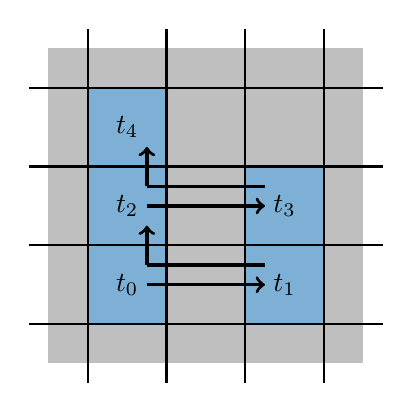
\begin{tikzpicture}[thick]
    \fill[gray!50](0.5,0.5) rectangle (4.5, 4.5); ;
    \draw[step=1 cm, color=black] (0.25, 0.25) grid (4.75, 4.75);
    
    \node[fill=omni-spring-pastels-2, minimum size=1 cm, draw=black] (1) at (1.5, 1.5) {\textbf{$t_0$}};
    \node[fill=omni-spring-pastels-2, minimum size=1 cm, draw=black] (3) at (3.5, 1.5) {\textbf{$t_1$}};
    \node[fill=omni-spring-pastels-2, minimum size=1 cm, draw=black] (2) at (1.5, 2.5) {\textbf{$t_2$}};
    \node[fill=omni-spring-pastels-2, minimum size=1 cm, draw=black] (4) at (3.5, 2.5) {\textbf{$t_3$}};
    \node[fill=omni-spring-pastels-2, minimum size=1 cm, draw=black] (5) at (1.5, 3.5) {\textbf{$t_4$}};

    \coordinate (4t2) at (1.75, 1.5) ;
    \coordinate (2f4) at (3.25, 1.5) ;
    \draw[->, very thick] (4t2) -- (2f4);

    \coordinate (2t4t2) at (3.25, 1.75) ;
    \coordinate (4f2)   at (1.75, 1.75) ;
    \coordinate (1f4f2) at (1.75, 2.25) ;
    \draw[-, very thick] (2t4t2) -- (4f2);
    \draw[->, very thick] (4f2) -- (1f4f2);

    \coordinate (1t0) at (1.75, 2.5) ;
    \coordinate (0f1) at (3.25, 2.5) ;
    \draw[->, very thick] (1t0) -- (0f1);
    
    \coordinate (0t1t3) at (3.25, 2.75) ;
    \coordinate (1f0)   at (1.75, 2.75) ;
    \coordinate (3f1f0) at (1.75, 3.25) ;
    \draw[-, very thick] (0t1t3) -- (1f0);
    \draw[->, very thick] (1f0) -- (3f1f0);

\end{tikzpicture}

            }
        \end{figure}
    \end{columns}
\end{frame}

\begin{frame}{Application profile}
    \centering Communication behavior

    \begin{figure}[!ht]
        \centering
        \resizebox{.75\linewidth}{!}{
            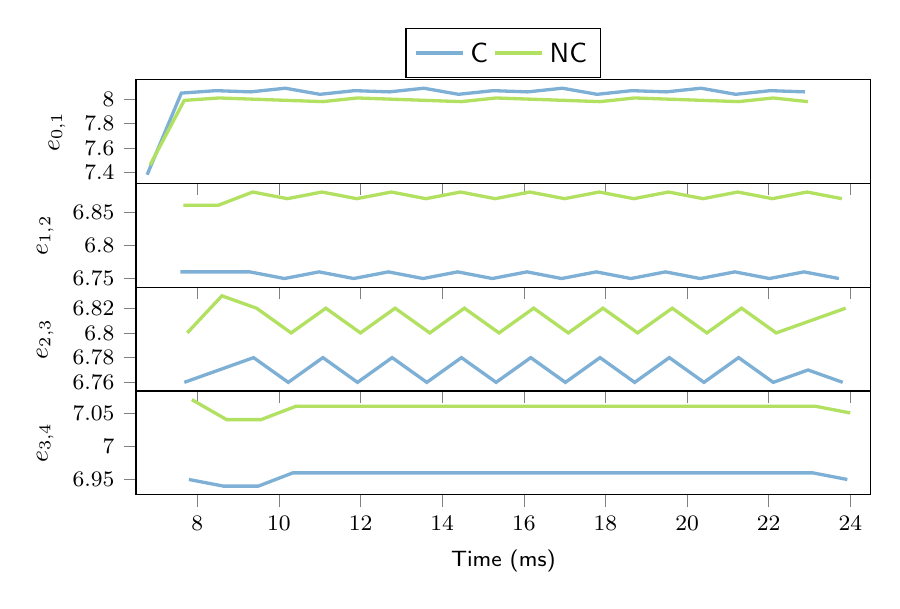
\begin{tikzpicture}
    \begin{groupplot}[
        group style={
            group name=my plots,
            group size=1 by 4,
            xlabels at=edge bottom,
            xticklabels at=edge bottom,
            vertical sep=0pt
        },
        small,
        width=.9\linewidth,
        height=2.9cm,
        xlabel={\footnotesize Time (ms)},
        xmin=6.5, xmax=24.5,
        % grid=major,
        tickpos=left,
        ytick align=outside,
        xtick align=outside,
    ]
        \nextgroupplot [
            ylabel={$e_{0,1}$ \scriptsize}, 
            legend style={
                at={(0.5,1.5)}, 
                anchor=north,
                legend columns=3
            },
        ]
        \addplot+ [mark=none, omni-spring-pastels-2, very thick] coordinates{
            (6.7724, 7.38)
            (7.61006, 8.05)
            (8.45949, 8.07)
            (9.30819, 8.06)
            (10.15691, 8.09)
            (11.00561, 8.04)
            (11.85433, 8.07)
            (12.70303, 8.06)
            (13.55175, 8.09)
            (14.40045, 8.04)
            (15.24917, 8.07)
            (16.09787, 8.06)
            (16.94659, 8.09)
            (17.79529, 8.04)
            (18.64401, 8.07)
            (19.49271, 8.06)
            (20.34143, 8.09)
            (21.19013, 8.04)
            (22.03885, 8.07)
            (22.88755, 8.06)        
        };

        \addplot+ [mark=none, omni-spring-pastels-3, very thick] coordinates{
            (6.84402, 7.46)
            (7.68168, 7.99)
            (8.53111, 8.01)
            (9.37981, 8.0)
            (10.22853, 7.99)
            (11.07723, 7.98)
            (11.92595, 8.01)
            (12.77465, 8.0)
            (13.62337, 7.99)
            (14.47207, 7.98)
            (15.32079, 8.01)
            (16.16949, 8.0)
            (17.01821, 7.99)
            (17.86691, 7.98)
            (18.71563, 8.01)
            (19.56433, 8.0)
            (20.41305, 7.99)
            (21.26175, 7.98)
            (22.11047, 8.01)
            (22.95917, 7.98)
        };

        \legend{\strut C, \strut NC}
        
        \nextgroupplot [ylabel={$e_{1,2}$ \scriptsize}]
        \addplot+ [mark=none, omni-spring-pastels-2, very thick] coordinates{
            (7.58932, 6.76)
            (8.43875, 6.76)
            (9.28745, 6.76)
            (10.13616, 6.75)
            (10.98487, 6.76)
            (11.83358, 6.75)
            (12.68229, 6.76)
            (13.531, 6.75)
            (14.37971, 6.76)
            (15.22842, 6.75)
            (16.07713, 6.76)
            (16.92584, 6.75)
            (17.77455, 6.76)
            (18.62326, 6.75)
            (19.47197, 6.76)
            (20.32068, 6.75)
            (21.16939, 6.76)
            (22.0181, 6.75)
            (22.86681, 6.76)
            (23.72004, 6.75)
        };

        \addplot+ [mark=none, omni-spring-pastels-3, very thick] coordinates{
            (7.66104, 6.86)
            (8.51047, 6.86)
            (9.35919, 6.88)
            (10.2079, 6.87)
            (11.05661, 6.88)
            (11.90532, 6.87)
            (12.75403, 6.88)
            (13.60274, 6.87)
            (14.45145, 6.88)
            (15.30016, 6.87)
            (16.14887, 6.88)
            (16.99758, 6.87)
            (17.84629, 6.88)
            (18.695, 6.87)
            (19.54371, 6.88)
            (20.39242, 6.87)
            (21.24113, 6.88)
            (22.08984, 6.87)
            (22.93855, 6.88)
            (23.79178, 6.87)
        };
        
        \nextgroupplot [ylabel={$e_{2,3}$}] %[ylabel={\footnotesize Latency (us)}, ylabel shift = -30 pt, every axis y label/.append style={at=(ticklabel cs:1.0)}]
        \addplot+ [mark=none, omni-spring-pastels-2, very thick] coordinates{
            (7.68254, 6.76)
            (8.5323, 6.77)
            (9.38028, 6.78)
            (10.22899, 6.76)
            (11.0777, 6.78)
            (11.92641, 6.76)
            (12.77512, 6.78)
            (13.62383, 6.76)
            (14.47254, 6.78)
            (15.32125, 6.76)
            (16.16996, 6.78)
            (17.01867, 6.76)
            (17.86738, 6.78)
            (18.71609, 6.76)
            (19.5648, 6.78)
            (20.41351, 6.76)
            (21.26222, 6.78)
            (22.11093, 6.76)
            (22.96415, 6.77)
            (23.81287, 6.76)
        };

        \addplot+ [mark=none, omni-spring-pastels-3, very thick] coordinates{
            (7.7543, 6.8)
            (8.60408, 6.83)
            (9.45206, 6.82)
            (10.30077, 6.8)
            (11.14948, 6.82)
            (11.99819, 6.8)
            (12.8469, 6.82)
            (13.69561, 6.8)
            (14.54432, 6.82)
            (15.39303, 6.8)
            (16.24174, 6.82)
            (17.09045, 6.8)
            (17.93916, 6.82)
            (18.78787, 6.8)
            (19.63658, 6.82)
            (20.48529, 6.8)
            (21.334, 6.82)
            (22.18271, 6.8)
            (23.03593, 6.81)
            (23.88467, 6.82)
        };

        \nextgroupplot [ylabel={$e_{3,4}$ \scriptsize}]
        \addplot+ [mark=none, omni-spring-pastels-2, very thick] coordinates{
            (7.79647, 6.95)
            (8.64654, 6.94)
            (9.49379, 6.94)
            (10.34254, 6.96)
            (11.19123, 6.96)
            (12.03996, 6.96)
            (12.88865, 6.96)
            (13.73738, 6.96)
            (14.58607, 6.96)
            (15.4348, 6.96)
            (16.28349, 6.96)
            (17.13222, 6.96)
            (17.98091, 6.96)
            (18.82964, 6.96)
            (19.67833, 6.96)
            (20.52706, 6.96)
            (21.37575, 6.96)
            (22.22448, 6.96)
            (23.07768, 6.96)
            (23.92641, 6.95)
        };

        \addplot+ [mark=none, omni-spring-pastels-3, very thick] coordinates{
            (7.86835, 7.07)
            (8.71842, 7.04)
            (9.56567, 7.04)
            (10.41442, 7.06)
            (11.26311, 7.06)
            (12.11184, 7.06)
            (12.96053, 7.06)
            (13.80926, 7.06)
            (14.65795, 7.06)
            (15.50668, 7.06)
            (16.35537, 7.06)
            (17.2041, 7.06)
            (18.05279, 7.06)
            (18.90152, 7.06)
            (19.75021, 7.06)
            (20.59894, 7.06)
            (21.44763, 7.06)
            (22.29636, 7.06)
            (23.14956, 7.06)
            (23.99831, 7.05)
        };
        
    \end{groupplot}    
\end{tikzpicture}

        }
    \end{figure}
\end{frame}

\begin{frame}{Application profile}
    \centering Mapping with Disturbing traffic
    \begin{figure}
        \centering
        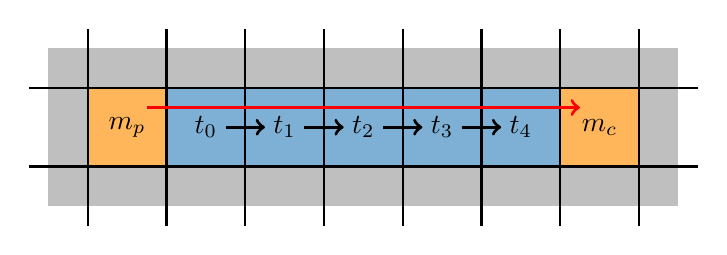
\begin{tikzpicture}[thick]

    \fill[gray!50](0.5,0.5) rectangle (8.5, 2.5); ;
    \draw[step=1 cm, color=black] (0.25, 0.25) grid (8.75, 2.75);
    
    \node[fill=omni-spring-pastels-2, minimum size=1 cm, draw=black] (1) at (2.5, 1.5) {\textbf{$t_0$}};
    \node[fill=omni-spring-pastels-2, minimum size=1 cm, draw=black] (3) at (3.5, 1.5) {\textbf{$t_1$}};
    \node[fill=omni-spring-pastels-2, minimum size=1 cm, draw=black] (2) at (4.5, 1.5) {\textbf{$t_2$}};
    \node[fill=omni-spring-pastels-2, minimum size=1 cm, draw=black] (4) at (5.5, 1.5) {\textbf{$t_3$}};
    \node[fill=omni-spring-pastels-2, minimum size=1 cm, draw=black] (5) at (6.5, 1.5) {\textbf{$t_4$}};
    

    \coordinate (4t2) at (2.75, 1.5) ;
    \coordinate (2f4) at (3.25, 1.5) ;
    \draw[->, very thick] (4t2) -- (2f4);
    
    \coordinate (2t1) at (3.75, 1.5) ;
    \coordinate (1f2) at (4.25, 1.5) ;
    \draw[->, very thick] (2t1) -- (1f2);

    \coordinate (1t0) at (4.75, 1.5) ;
    \coordinate (0f1) at (5.25, 1.5) ;
    \draw[->, very thick] (1t0) -- (0f1);
    
    
    \coordinate (0t3) at (5.75, 1.5) ;
    \coordinate (3f0) at (6.25, 1.5) ;
    \draw[->, very thick] (0t3) -- (3f0);

    \node[fill=omni-spring-pastels-5, minimum size=1 cm, draw=black] (6) at (1.5, 1.5) {\textbf{$m_p$}};
    \node[fill=omni-spring-pastels-5, minimum size=1 cm, draw=black] (7) at (7.5, 1.5) {\textbf{$m_c$}};

    \coordinate (ptc) at (1.75, 1.75) ;
    \coordinate (cfp) at (7.25, 1.75) ;
    \draw[red, ->, very thick] (ptc) -- (cfp);
\end{tikzpicture}

    \end{figure}

    \begin{itemize}
        \item $m_p$ sends messages to $m_c$
        \item Random intervals (100-500 $\mu s$)
        \item 96 flits per message        
    \end{itemize}
\end{frame}

\begin{frame}{Application profiling}
    \centering Communication behavior

    \begin{figure}[!ht]
        \centering
        \resizebox{0.75\linewidth}{!}{
            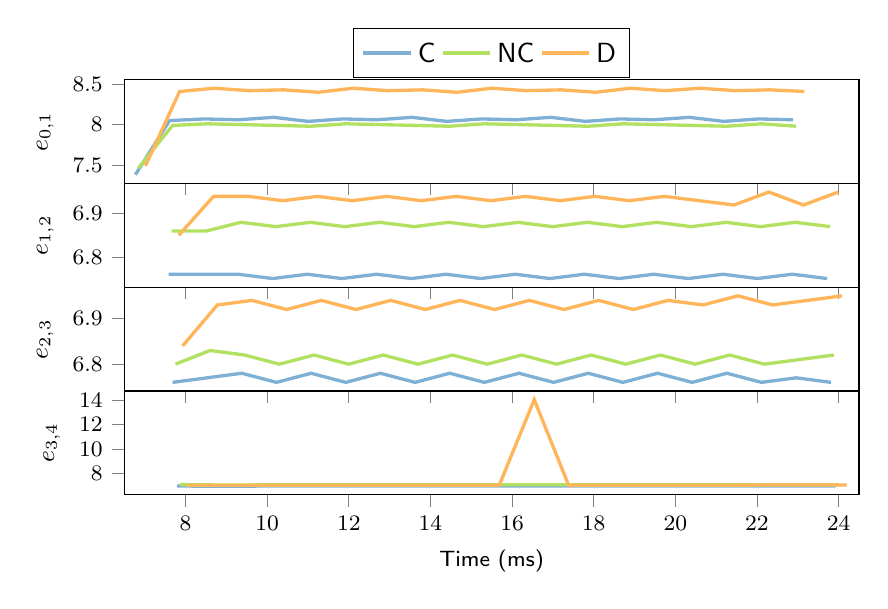
\begin{tikzpicture}
    \begin{groupplot}[
        group style={
            group name=my plots,
            group size=1 by 4,
            xlabels at=edge bottom,
            xticklabels at=edge bottom,
            vertical sep=0pt
        },
        small,
        width=.9\linewidth,
        height=2.9cm,
        xlabel={\footnotesize Time (ms)},
        xmin=6.5, xmax=24.5,
        % grid=major,
        tickpos=left,
        ytick align=outside,
        xtick align=outside,
    ]
        \nextgroupplot [
            ylabel={$e_{0,1}$ \scriptsize}, 
            legend style={
                at={(0.5,1.5)}, 
                anchor=north,
                legend columns=3
            },
        ]
        \addplot+ [mark=none, omni-spring-pastels-2, very thick] coordinates{
            (6.7724, 7.38)
            (7.61006, 8.05)
            (8.45949, 8.07)
            (9.30819, 8.06)
            (10.15691, 8.09)
            (11.00561, 8.04)
            (11.85433, 8.07)
            (12.70303, 8.06)
            (13.55175, 8.09)
            (14.40045, 8.04)
            (15.24917, 8.07)
            (16.09787, 8.06)
            (16.94659, 8.09)
            (17.79529, 8.04)
            (18.64401, 8.07)
            (19.49271, 8.06)
            (20.34143, 8.09)
            (21.19013, 8.04)
            (22.03885, 8.07)
            (22.88755, 8.06)        
        };

        \addplot+ [mark=none, omni-spring-pastels-3, very thick] coordinates{
            (6.84402, 7.46)
            (7.68168, 7.99)
            (8.53111, 8.01)
            (9.37981, 8.0)
            (10.22853, 7.99)
            (11.07723, 7.98)
            (11.92595, 8.01)
            (12.77465, 8.0)
            (13.62337, 7.99)
            (14.47207, 7.98)
            (15.32079, 8.01)
            (16.16949, 8.0)
            (17.01821, 7.99)
            (17.86691, 7.98)
            (18.71563, 8.01)
            (19.56433, 8.0)
            (20.41305, 7.99)
            (21.26175, 7.98)
            (22.11047, 8.01)
            (22.95917, 7.98)
        };

        \addplot+ [mark=none, omni-spring-pastels-5, very thick] coordinates{
            (7.01808, 7.49)
            (7.85639, 8.41)
            (8.707, 8.45)
            (9.55634, 8.42)
            (10.4057, 8.43)
            (11.25504, 8.4)
            (12.1044, 8.45)
            (12.95374, 8.42)
            (13.8031, 8.43)
            (14.65244, 8.4)
            (15.5018, 8.45)
            (16.35114, 8.42)
            (17.2005, 8.43)
            (18.04984, 8.4)
            (18.8992, 8.45)
            (19.74854, 8.42)
            (20.60694, 8.45)
            (21.46152, 8.42)
            (22.31088, 8.43)
            (23.16022, 8.41)
        };

        \legend{\strut C, \strut NC, \strut D}
        
        \nextgroupplot [ylabel={$e_{1,2}$ \scriptsize}]
        \addplot+ [mark=none, omni-spring-pastels-2, very thick] coordinates{
            (7.58932, 6.76)
            (8.43875, 6.76)
            (9.28745, 6.76)
            (10.13616, 6.75)
            (10.98487, 6.76)
            (11.83358, 6.75)
            (12.68229, 6.76)
            (13.531, 6.75)
            (14.37971, 6.76)
            (15.22842, 6.75)
            (16.07713, 6.76)
            (16.92584, 6.75)
            (17.77455, 6.76)
            (18.62326, 6.75)
            (19.47197, 6.76)
            (20.32068, 6.75)
            (21.16939, 6.76)
            (22.0181, 6.75)
            (22.86681, 6.76)
            (23.72004, 6.75)
        };

        \addplot+ [mark=none, omni-spring-pastels-3, very thick] coordinates{
            (7.66104, 6.86)
            (8.51047, 6.86)
            (9.35919, 6.88)
            (10.2079, 6.87)
            (11.05661, 6.88)
            (11.90532, 6.87)
            (12.75403, 6.88)
            (13.60274, 6.87)
            (14.45145, 6.88)
            (15.30016, 6.87)
            (16.14887, 6.88)
            (16.99758, 6.87)
            (17.84629, 6.88)
            (18.695, 6.87)
            (19.54371, 6.88)
            (20.39242, 6.87)
            (21.24113, 6.88)
            (22.08984, 6.87)
            (22.93855, 6.88)
            (23.79178, 6.87)
        };

        \addplot+ [mark=none, omni-spring-pastels-5, very thick] coordinates{
            (7.83542, 6.85)
            (8.68612, 6.94)
            (9.53546, 6.94)
            (10.38481, 6.93)
            (11.23416, 6.94)
            (12.08351, 6.93)
            (12.93286, 6.94)
            (13.78221, 6.93)
            (14.63156, 6.94)
            (15.48091, 6.93)
            (16.33026, 6.94)
            (17.17961, 6.93)
            (18.02896, 6.94)
            (18.87831, 6.93)
            (19.72766, 6.94)
            (20.58605, 6.93)
            (21.44062, 6.92)
            (22.29001, 6.95)
            (23.13932, 6.92)
            (23.99323, 6.95)
        };
        
        \nextgroupplot [ylabel={$e_{2,3}$}] %[ylabel={\footnotesize Latency (us)}, ylabel shift = -30 pt, every axis y label/.append style={at=(ticklabel cs:1.0)}]
        \addplot+ [mark=none, omni-spring-pastels-2, very thick] coordinates{
            (7.68254, 6.76)
            (8.5323, 6.77)
            (9.38028, 6.78)
            (10.22899, 6.76)
            (11.0777, 6.78)
            (11.92641, 6.76)
            (12.77512, 6.78)
            (13.62383, 6.76)
            (14.47254, 6.78)
            (15.32125, 6.76)
            (16.16996, 6.78)
            (17.01867, 6.76)
            (17.86738, 6.78)
            (18.71609, 6.76)
            (19.5648, 6.78)
            (20.41351, 6.76)
            (21.26222, 6.78)
            (22.11093, 6.76)
            (22.96415, 6.77)
            (23.81287, 6.76)
        };

        \addplot+ [mark=none, omni-spring-pastels-3, very thick] coordinates{
            (7.7543, 6.8)
            (8.60408, 6.83)
            (9.45206, 6.82)
            (10.30077, 6.8)
            (11.14948, 6.82)
            (11.99819, 6.8)
            (12.8469, 6.82)
            (13.69561, 6.8)
            (14.54432, 6.82)
            (15.39303, 6.8)
            (16.24174, 6.82)
            (17.09045, 6.8)
            (17.93916, 6.82)
            (18.78787, 6.8)
            (19.63658, 6.82)
            (20.48529, 6.8)
            (21.334, 6.82)
            (22.18271, 6.8)
            (23.03593, 6.81)
            (23.88467, 6.82)
        };

        \addplot+ [mark=none, omni-spring-pastels-5, very thick] coordinates{
            (7.92905, 6.84)
            (8.78027, 6.93)
            (9.62835, 6.94)
            (10.4777, 6.92)
            (11.32705, 6.94)
            (12.1764, 6.92)
            (13.02575, 6.94)
            (13.8751, 6.92)
            (14.72445, 6.94)
            (15.5738, 6.92)
            (16.42315, 6.94)
            (17.2725, 6.92)
            (18.12185, 6.94)
            (18.9712, 6.92)
            (19.82055, 6.94)
            (20.67895, 6.93)
            (21.53352, 6.95)
            (22.38291, 6.93)
            (23.23673, 6.94)
            (24.08615, 6.95)
        };

        \nextgroupplot [ylabel={$e_{3,4}$ \scriptsize}]
        \addplot+ [mark=none, omni-spring-pastels-2, very thick] coordinates{
            (7.79647, 6.95)
            (8.64654, 6.94)
            (9.49379, 6.94)
            (10.34254, 6.96)
            (11.19123, 6.96)
            (12.03996, 6.96)
            (12.88865, 6.96)
            (13.73738, 6.96)
            (14.58607, 6.96)
            (15.4348, 6.96)
            (16.28349, 6.96)
            (17.13222, 6.96)
            (17.98091, 6.96)
            (18.82964, 6.96)
            (19.67833, 6.96)
            (20.52706, 6.96)
            (21.37575, 6.96)
            (22.22448, 6.96)
            (23.07768, 6.96)
            (23.92641, 6.95)
        };

        \addplot+ [mark=none, omni-spring-pastels-3, very thick] coordinates{
            (7.86835, 7.07)
            (8.71842, 7.04)
            (9.56567, 7.04)
            (10.41442, 7.06)
            (11.26311, 7.06)
            (12.11184, 7.06)
            (12.96053, 7.06)
            (13.80926, 7.06)
            (14.65795, 7.06)
            (15.50668, 7.06)
            (16.35537, 7.06)
            (17.2041, 7.06)
            (18.05279, 7.06)
            (18.90152, 7.06)
            (19.75021, 7.06)
            (20.59894, 7.06)
            (21.44763, 7.06)
            (22.29636, 7.06)
            (23.14956, 7.06)
            (23.99831, 7.05)
        };

        \addplot+ [mark=none, omni-spring-pastels-5, very thick] coordinates{
            (8.04348, 7.01)
            (8.89503, 7.02)
            (9.74184, 7.02)
            (10.59121, 7.02)
            (11.44054, 7.02)
            (12.28991, 7.02)
            (13.13924, 7.02)
            (13.98861, 7.02)
            (14.83794, 7.02)
            (15.68731, 7.02)
            (16.54366, 14.04)
            (17.38601, 7.02)
            (18.23534, 7.02)
            (19.08471, 7.02)
            (19.93404, 7.02)
            (20.79246, 7.02)
            (21.64701, 7.02)
            (22.49644, 7.04)
            (23.35024, 7.04)
            (24.19967, 7.03)
        };
        
    \end{groupplot}    
\end{tikzpicture}

        }
    \end{figure}
\end{frame}

\begin{frame}{Application profile}
    \begin{itemize}
        \item An application has a communication behavior for each of its edges
        \item The behavior does not change with the number of hops between edges
    \end{itemize}

    \vspace{0.5cm}
    \textit{This behavior cannot be captured by models that only monitor latency, which was adopted in early work}

    \begin{alertblock}{Challenge}
        Develop an application profile capable of monitoring the latency of each edge in the NoC to detect potential malicious interferences using ML
    \end{alertblock}
\end{frame}
\section{A Framework for Pre-Runtime RT Analysis}

\begin{frame}{Overview}
	\begin{itemize}
		\item We propose a framework to identify whether a NoC-based manycore can run a real-time application without deadline violations. 
		
		\item We implemented a couple of tools to automate our approach, which relies on the \textit{scheduling} of system resources --- computation and communication. 
		
		\item Scheduling tasks on a single-core CPU is not novel, as some existing solutions date back to the 80s~\cite{gusfield:1984}. 
		
		\item However, incorporating the I/O components of the system, managing interruptions, and addressing the needs of NoCs requires additional modeling.
	\end{itemize}
\end{frame}

\begin{frame}
	\begin{itemize}
	\item Our framework concerns dataflow applications, where tasks have data dependency on sensors, the network, data off-loading, or other tasks. 
	
	\item In addition, tasks must employ a variation of the predictable execution (PREM)~\cite{Senoussaoui:2022} and the logical execution time (LET)~\cite{Gemlau:2021} models; we divide tasks in \emph{receiving}, \emph{processing}, and \emph{sending} phases as the controlled execution of tasks is key for I/O access predictability. 
	
	\item We expect applications to have real-time requirements on (i) the iteration time and (ii) the number of iterations per second. The former is the end-to-end application execution time, which is particularly important in sensor applications as it dictates the accuracy of sensors in time, i.e., how old the reading is. The latter is the application execution rate, which relates to the periodic execution of tasks.
	\end{itemize}
\end{frame}

\begin{frame}
	\begin{figure}[!t]
		\centerline{\includegraphics[width=0.8\columnwidth]{fig/workflow.pdf}}
		\caption{A workflow depicting our approach. User inputs appear at the top. Activities appear as blue shapes. Outcomes appear as green shapes. Tags A, B, and C represent activities of the workflow that may fail due to the unavailability of system resources. Tag D represents the end of the workflow, where users can choose to abandon the workflow or further optimize the result.}
		\label{fig:workflow}
		\vspace{-12 pt}
	\end{figure}
\end{frame}

\begin{frame}

	The proposed framework (Figure~\ref{fig:workflow}) takes three inputs: (i) application graph, (ii) architecture specification, and (iii) nominal manycore frequency. 
	
	\begin{enumerate}
		\item[i)] We described applications using a directed, potentially cyclic, graph $G = (E, V)$, where $V$ is the set of vertices and $E$ is the set of edges. Vertices represent tasks, to which we tag the corresponding worst-case execution time (WCET), in cycles. Edges represent flows of data, i.e., a set of packets with periodic behavior, given by a $3$-tuple $f =\langle p, c, d \rangle$, corresponding to the period ($p$), capacity ($c$), and deadline of flows ($d)$, in clock cycles.
		\item[ii)] The architecture specification must describe a zero-load latency model of the network and a set of allowed operating frequencies for the manycore. Please note that the entire system runs at the same frequency.
		\item[iii)] The framework considers the nominal frequency as the start point for the frequency optimization. 
	\end{enumerate}
\end{frame}

\begin{frame}

	\begin{itemize}
		\item At the first iteration, the framework computes whether the nominal frequency suits the application. 
		
		\item The framework runs in interactive or automated modes. 
		
		\item In interactive mode, users must decide to increase the frequency (if the platform allows), try a lower frequency, or abandon the process at each iteration. 
		
		\item In automated mode, the framework runs until it reaches a given number of iterations or cannot optimize the frequency further, assuming a tolerance factor. 
		
		\item The framework evaluates the application at each iteration, using a 5-step analysis: (i) task clustering, (ii) task mapping, (iii) application instantiation, (iv) CPU analysis, and (v) network analysis. CPU analysis splits in critical path analysis (CPA) and CPU simulation.
	\end{itemize}

\end{frame}

% -------------------------------------------------------------------------------


\begin{frame}{1 - Task Set Clustering and Mapping}
	\begin{itemize}
	\item Task set clustering consists of splitting an application graph into multiple task sets to be assigned by the framework to a PE during the mapping step (Figure~\ref{fig:workflow}, step 1). 
	
	\item The goal is to generate one cluster per PE. We created an algorithm to cluster graphs that performs $O(n)$  on the number of vertices of the application task graph. 
	
	\item The algorithm iteratively removes edges from the graph, combining vertices until the resulting graph has $|$\textit{V}$| \leq |\text{\textit{PEs}}|$, based on one of two criteria. 
	
	\item The \textsc{min-comm} criterion reduces the overall network load, eliminating edges with the most communication load groups communication-intensive tasks in the same cluster. 
	
	\item Oppositely, the \textsc{max-proc} criterion balances the CPU usage between PEs by grouping tasks with the least CPU load. Once the algorithm computes the clusters, we can map them to the manycore using a task mapping strategy (Figure~\ref{fig:workflow}, step 2). 
	
	\item Note that task mapping is a well-developed topic in the literature~\cite{Singh:2013}, so discussing task mapping is out of the scope of this paper.
	\end{itemize}
\end{frame}

\begin{frame}{2 - Application Instantiation and Framework Loop}
	\begin{itemize}
		\item As the framework explores different frequencies during its execution, it must adjust the application parameters to match the frequency at each iteration (Figure~\ref{fig:workflow}, step 3). 
		
		\item The framework carries the WCET value of tasks along the multiple iterations, as the CPU architecture does not change. However, the framework must consider the periodicity of flows, adjusting the period and deadline of flows accordingly. 
		
		\item Iterations occur as follows. At the first iteration, the framework takes the nominal frequency as the candidate frequency, employing no adjustments to the application. 
		
		\item Based on the results of CPU analysis (Figure~\ref{fig:workflow}, step 4) and network analysis (Figure~\ref{fig:workflow}, step 5), the framework either increases or decreases the frequency. If the framework identifies violations of deadlines (tasks or flows), the candidate frequency will increase at the next iteration. 
		
		\item Similarly, the framework reduces the frequency if it detects no deadline violations. Searching for the minimum feasible frequency performs $O(log \ n)$, i.e., the time complexity of the binary search, where $n$ is the number of frequencies supported by the target platform (discrete).%GRAMMARLY-OK
	\end{itemize}
\end{frame}



\begin{frame}{3.a - Critical Path Analysis (CPA)}
	
	\begin{itemize}
		\item The CPU analysis is a 2-step process to assert that the manycore meets the CPU needs of an application. 
		
		\item The framework uses the CPA method~\cite{Kelley:1959} to evaluate the end-to-end processing time of an application iteration (Figure~\ref{fig:workflow}, step 4.1). 
		
		\item As PEs carry only subsets of the application task set, we must account for internal communication (task-to-task communication through memory spaces) and external communication (NoC). 
		
		\item The CPA method proceeds as Djkistra’s algorithm for computing the shortest path between two vertices~\cite{dijkstra:1959}, except that we multiply the weights of edges (communication load) by $-1$. 
		
		\item Although we cannot apply topological sort to cyclic graphs, we use depth-first search (DFS) to find and remove cycles, adding the weight of a removed edge to its origin vertex. 
		
		\item The result of this step is the number of cycles that the application takes to execute, i.e., the iteration time. The CPU must have enough cycles to run the application. Otherwise, the framework discards the candidate frequency and moves on to the next iteration.%GRAMMARLY-OK
	\end{itemize}
\end{frame}


\begin{frame}{3.b - Discrete-Event Simulation (DES) of PEs}
	
	\begin{itemize}
		
		\item The execution time of some kernel routines, e.g., dynamic memory allocation (\textit{malloc}) and interruption handling, is hard to predict. Our framework uses a DES engine to simulate PEs while assuming a worst-case characterization of kernel operations (Figure~\ref{fig:workflow}, step 4.2).
		
		\item It simulates PEs individually to find whether they can run the assigned task cluster. The simulation considers the WCET of the task scheduler, I/O interrupts, and other minor system-specific programmable interrupts. 
		
		\item If the framework detects that one of the PEs cannot run the assigned task set, the framework discards the candidate frequency and moves to the next iteration. 
		
		\item Due to the employment of the PREM and LET models, the framework can estimate the time in which tasks inject packets into the network. Packets enter the network only at the \textit{sending} phase, triggering an I/O event in the kernel. 
		
		\item The framework uses these values during the network analysis step (Figure~\ref{fig:workflow}, step 5) to predict the behavior of packets.
		
	\end{itemize}

\end{frame}



\begin{frame}{4 - Network Analysis}
	
	\begin{itemize}
		\item The network analysis occurs after the CPU analysis, considering that the framework kept the candidate frequency. 
		
		\item In this step, the framework asserts whether the network flows can traverse the NoC without deadline violations for a static set of flows. 
		
		\item Our flow model reassembles the Job-Shop model~\cite{Garey:1979}, where we replace machines with links (channels) and jobs with flits (data units). The goal of the network analysis step is to find a schedule for packets. The network analysis has 3 steps:
		
	\end{itemize}
\end{frame}

\begin{frame}{4 - Network Analysis (contd.)}
	
	
	\begin{enumerate}
		\item Unwrap flows to packets $p = \langle mrt, size, ad \rangle$, having a minimum release time ($mrt$), data size ($size$), and absolute deadline ($ad$) each. 
		
		\item Discover the path of packets in the NoC to compute the occupancy of links ($L$), i.e., a relation $O : P \times L \times T$, matching packets to the links they occupy in the discrete time domain (cycles), where $\forall p \in P$. 
		
		\item Find a schedule where the following constraints hold:
		\begin{itemize}
			\item[(\textsc{c1})] $prt \geq mrt$, where $ptr$ is the release time of packets in the found schedule;
			\item[(\textsc{c2})] $ad \geq prt + size / lw$, where $lw$ is the link width;
			\item[(\textsc{c3})] packets cannot overlap (single channel constraint);
			\item[(\textsc{c4})] flits of a same packet occupy the data bus one after another (wormhole constraint). 
			
		\end{itemize}
	\end{enumerate}
\end{frame}

\begin{frame}{Beware!}
	
	\begin{itemize}
		\item Generating a network schedule is NP-complete (similarly to job-shop).
		
		\item Instead, we use the $prt$ values collected during the CPU analysis, reducing the scheduling to a decision problem. 
		
		\item The framework indicates whether the schedule is feasible or not. If the schedule is feasible, the framework \textit{memorizes} the minimum frequency found so far. 
		
		\item Then, the framework can either try to find a lower frequency or abandon the process.%GRAMMARLY-OK
	\end{itemize}
	
\end{frame}
\section{Proof-of-Concept and Results}

\begin{frame}{Experimentation Setup}
  
  \begin{itemize}
  	\item We experiment on the SAE (synthetic) application whose minimum frequency to meet its RT requirements is known ($500$MHz).
  	\item We map SAE to a 2x2 instance of our manycore
	\item We perform clustering using the \textit{max-proc} criterion and $n = 4$.
	\item The nominal frequency of our platform is $2.5$GHz, which is also given as input to our framework. 
	\item By the last iteration, our framework found $500.4$MHz as the minimum frequency to meet the RT constraints on the platform. Since we cannot display the results for all iterations, we couple to show the last step and demonstrate how the found frequency meets the requirement of the application (the last frequency).
  \end{itemize}
  
\end{frame}


\begin{frame}
	
	\begin{itemize}
		\item The CPA method estimated the end-to-end iteration execution time of SAE based on the application graph and the WCET of the kernel operations. 
		
		\item Our scheduler has a WCET of $110$ kcycles, and our network driver has a WCET of $20$ kcycles. Tasks are scheduled once per iteration due to our PBRR implementation. The total iteration execution time, as pointed out by the CPA method, is $8.464.895$ cycles. 
		
		\item The actual RTL execution is $6.799.200$ cycles ($80\%$). The CPA method overestimates $\simeq 26\%$ of the actual CPU usage. However, the overestimation is \textit{acceptable} ($<30\%$) as the actual CPU usage stays below  $70\%$; a CPU usage over $70\%$ is often considered questionable~\cite{Ovaska:2011}.
		
	\end{itemize}
	

\end{frame}

\begin{frame}{}
    
    \vspace{-0.8em}
    \begin{table}[!ht]
    	\caption{Comparison of Execution time (CPU).}
    	\label{tab:results}
    	\centering
    	\resizebox{1\textwidth}{!}{%
    		\begin{tabular}{lrrrrr}
    			\toprule
    			\textbf{Cluster} & \textbf{Execution$^1$} & \textbf{Estimation$^2$} & \textbf{Difference} & \textbf{Diff. (\%)$^3$} & \textbf{Usage$^4$}\\
    			\cmidrule(lr){1-1}
    			\cmidrule(lr){2-2}
    			\cmidrule(lr){3-3}
    			\cmidrule(lr){4-4}
    			\cmidrule(lr){5-5}
    			\cmidrule(lr){6-6}
    			
    			\rowcolor{\rowcolordark} 
    			ABDF & $1,439,000$ & $1,819,300$ & $+380,300$ & $+26.428\%$ & $72.722\%$\\
    			
    			C & $801,300$ & $963,300$ & $+162.000$ & $+20.217\%$  & $38.532\%$\\
    			
    			\rowcolor{\rowcolordark} 
    			EHI & $2,174,500$ & $2,667,895$ & $+493,395$ &  $+22.690\%$  & $71.616\%$\\
    			
    			GJ & $2,384,400$ & $3,014,400$ & $+630.000$ & $+26.421\%$ & $86.980\%$\\     
    			
    			\bottomrule
    			\multicolumn{6}{p{9.5cm}}{\footnotesize{$^1$Execution time (RTL, cycles); $^2$CPA estimation; $^3$Execution time is $100\%$; $^4$DES.}}
    		\end{tabular}
    		
    	} % end of resize box
    \end{table}
    \vspace{-0.8em}
\end{frame}


\begin{frame}
	
	\begin{itemize}
		
		\item The framework captured the time that tasks finished during the DES simulation. As tasks implement the PREM and LET models, we assume that packets are injected at the same time they leave the CPU.
		
		\item Table~\ref{tab:flows} shows the characterization of flows, where $ph$ is the phase time (the period of scheduling interrupts), $pv$ is the \textit{phase} of the task, and $\psi = (ph \times pv)$. 
		
		\item A phase corresponds to the alignment of application execution to the scheduler tick. For instance, the SAE application cannot finish before the $4^{th}$ phase due to the critical path traverses 4 tasks in the application graph. This is a necessary step, as the DES simulation does not account for task dependency. Deadlines match the end of the phase of the receiving task.%GRAMMARLY-OK
				
	\end{itemize}
	
\end{frame}



\begin{frame}
	
	
	\vspace{-10 pt}
	\begin{table}[!ht]
		\caption{Characterization of flows for the SAE application.}
		\label{tab:flows}
		\centering
		\resizebox{0.8\textwidth}{!}{%
			\begin{tabular}{lrccrr}
				\toprule
				\textbf{Flow} & \textbf{MRT$^1$} & \textbf{S} & \textbf{D} & \textbf{Volume} & \textbf{Deadline}\\
				\cmidrule(lr){1-1}
				\cmidrule(lr){2-2}
				\cmidrule(lr){3-3}
				\cmidrule(lr){4-4}
				\cmidrule(lr){5-5}
				\cmidrule(lr){6-6}
				
				\rowcolor{\rowcolordark} $F_1$ & $285300 + \psi$ & A & C & $12300$ & $110000 +  \psi$\\
				$F_2$ & $1819300 + \psi$ & F & G & $67800$ & $110000 + \psi$\\
				\rowcolor{\rowcolordark} $F_3$ & $963300  + \psi$ & C & E & $12000$ & $110000 + \psi$\\
				$F_4$ & $1280700 + \psi$ & I & J & $56700$ & $1208800  + \psi$\\
				\rowcolor{\rowcolordark} $F_5$ & $1733700 + \psi$ & H & J & $89000$ & $1208800 + \psi$\\
				
				\bottomrule
				\multicolumn{6}{p{7cm}}{\footnotesize{(S) source task, (D) destination task, $^1$Minimum release time.}}
			\end{tabular}
			
		} % end of resize box
		\vspace{-8 pt}
	\end{table}	
	
\end{frame}



\begin{frame}
	\begin{itemize}
		\item In Figure~\ref{fig:phases}, we present the RTL simulation of our manycore running the SAE application at the minimum frequency of $500.4$MHz, obtained from our framework. The goal is to demonstrate that the application meets its RT requirements. 
		
		\item The hyperperiod of SAE is $20$ms, corresponding to 4 phases of $5$ms each, meeting the expected iteration time and iterations per second requirements. SAE receives stimuli from outside the system once per $5$ms, triggering $4$ instances of the application per $20ms$ (Task \textsc{a}). SAE returns results to outside the system via Task \textsc{j}. 
		
		\item The $3^{\text{rd}}$ instance of the application (pink) has additional $1.457$ms in its iteration time, related to the scheduling of Task \textsc{i}; the task executes two iterations at once due to two packets received in the phase time, delaying Task \textsc{j}. Nevertheless, Task \textsc{j} meets its deadlines for all instances of SAE, for an iteration time of $16,820$ms for the $1^{\text{st}}$, $2^{\text{nd}}$ and $3^{\text{th}}$ instances, and $18.277$ms for the $3^{\text{rd}}$ instance.
	\end{itemize}
\end{frame}


\begin{frame}
	\begin{figure}[!ht]
		\centerline{\includegraphics[width=0.8\columnwidth]{fig/results.pdf}}
		\caption{Interaction of tasks of the SAE application during RTL simulation. Rectangles with the same color represent tasks in the same iteration (instances). Arrows indicate the direction of the communication. The yellow rectangle represents a phase overlapping.}
		\vspace{-16 pt}
		\label{fig:phases}
	\end{figure}
\end{frame}
\section{Conclusions and Acknowledgements}

\begin{frame}{Conclusion}

	\begin{itemize}
		\item This paper proposes a framework for asserting the RT properties of applications running on NoC-based, multitasking, private-memory manycores. 
		
		\item Our framework observes the computation and communication  aspects of the application, adjusting the frequency of the target platform to the minimum while allowing the application to meet its RT requirements. 
		
		\item We demonstrate our framework on the SAE application, running on our manycore. Our framework could reduce the manycore frequency without compromising the RT requirements of SAE.%GRAMMARLY-OK
	\end{itemize}

\end{frame}

\begin{frame}{Conclusion (contd.)}
	
	\begin{itemize}
	\item Our framework enables the exploration of RT at the pre-runtime, alleviating the effects of stacked NFRs in the design. We avoid modeling design-specific features in our framework, e.g., buffer, allowing our framework to suit virtually any NoC that provides a zero-load latency model. 
	
	\item Future works include 
	\begin{enumerate}

		\item evaluating our approach while considering multiple NFRs, e.g. area and energy requirements; 
		
		\item experiment with more complex applications~\cite{shi:2010}; 
		
		\item make use of dynamic voltage-frequency scaling (DVFS) to improve energy efficiency without compromising real-time performance, and (iv) improve the automation of the approach, e.g., integration with ModelSim.
		
	\end{enumerate}
	\end{itemize}


\end{frame}

\begin{frame}{Acknowledgement}
	
	\begin{itemize}
		\item This work was financed in part by Coordenação de Aperfeiçoamento de Pessoal de Nível Superior (CAPES), Finance Code 001; Conselho Nacional de Desenvolvimento Científico e Tecnológico (CNPq), 309605/2020-2 and 407829/2022-9; Fundação de Amparo à Pesquisa do Estado do Rio Grande do Sul (FAPERGS), 21/2551-0002047-4 and 23/2551-0002200-1.
	\end{itemize}

	
\end{frame}

\frame[plain]{\titlepage}

\begin{frame}[allowframebreaks]{References}
    \tiny
    \bibliographystyle{alpha}
    \bibliography{bibliography}
\end{frame}

\end{document}

